\documentclass{article}
\usepackage[margin=1in]{geometry}
\usepackage{../common}
\usepackage{amsmath}
\usepackage{../pagesetup}
\usepackage{listings}
\usepackage{graphicx}

\begin{document}
%\lecture{**LECTURE-NUMBER**}{**DATE**}{**LECTURER**}{**SCRIBE**}
\lecture{19}{November 13}{Sasha Rush}{Chang Liu, Jiafeng Chen, Alexander Lin}{Monte Carlo Basics}%% Add your scribe names!!

% \subsection{Loopy BP}
\subsection{History} 
We started with Monte Carlo in the past few lectures. The main method is to use draw samples from a proposal distribution and take sample average to approximate expectations.
\begin{align*}
    \E_{y \sim p(y|x)}[f(y)] & = \int p(y|x) f(y) dy \\
    & \approx \frac{1}{N} \sum_{n=1}^{N} f(\tilde{y}^{(n)})
\end{align*}

where $\tilde{y}^{(n)} \sim p(y|x)$. This approach requires the ability to sample $y \sim p(y|x)$.

\subsection{Univariate Case}
Let's start at the beginning:  We know $F(x) = p(y \leq x)$ and it is univariate. 




% some figure on the CDF and its inverse map
% TODO INCLUDE
% \FloatBarrier
% \begin{figure}
% \center
% \includegraphics[width=0.4\textwidth]{}
% \includegraphics[width=0.4\textwidth]{time_t1}
% \caption{Message passing example: left (incoming), right (outgoing)}
% \end{figure}

Assume we can compute $F^{-1}(u)$, then 
$$ p(F^{u}\leq x) = p(u\leq F(x)) = F(x) u$$
where $F$ is the CDF of $u \sim \text{Unif}(0,1)$. However, this works only for univariate case. What this means is that, is we wish to sample $y \sim F$ for some known CDF $F$, we need only to sample $U\sim \text{Unif}$ and transform the sample of uniform random variables through $F^{-1}$ to get a sample of $y$. Formally, 
\[
U \sim \text{Unif} \implies F^{-1}(U) \sim F 
\]
(This is known as the probability integral transform).

\subsection{Normal Samples}
We pursue the same strategy as in the univariate case. Given Uniform samples, we wish to apply some transform to obtain a sample of multivariate random variables of some distribution we are interested in. We execute this strategy for Normal random variables (this is known as the Box-Muller transformation). The upshot here is that to sample Normal random variables, we need only to sample Uniform random variables, which is much easier to do.

\paragraph{Box-Muller} Sample $z_1,z_2 \sim \text{Unif}[-1,1]$. Discard the points outside of the unit circle, so our sample of $\{(z_1,z_2)\}$ is uniform on the unit disk. We would like to transform each $(z_1,z_2)$ into some $(x_1,x_2) \sim \mathcal N(0,I)$. We want to find the right transform such that the Jacobian makes the following hold \[
\overbrace{p(x_1,x_2)}^{\text{Normal PDF}} = \overbrace{p(z_1,z_2)}^{\text{Unif disk PDF}} \left|\frac{\partial(z_1,z_2)}{\partial(x_1,x_2)}\right|.
\]
We may check that \begin{align*}
x_1 &= z_1 \left({\frac{-2\log r^2}{r^2}}\right)^{1/2}\\
x_2 &= z_2 \left({\frac{-2\log r^2}{r^2}}\right)^{1/2},
\end{align*}
where $r^2 = z_1^2 + z_2^2$, is the desired transform.

% By the change of variable formula, we can reparametrize $x$ in terms of $z$
% $$ p(x) = |\dfrac{dz}{dx}| p(z) $$ 
% where $z_1,z_2 \sim \text{Unif}(-1,1)$. 

% We will only keep samples in a circle such that $r^2 := z_1^2 + z_2^2 \leq 1$, and would like to draw samples $x_1,x_2 \sim N(0,1)$. 

% % insert figure of a circle in a square
% $$ p(x_1,x_2) = p(z_1,z_2 ) | \dfrac{d(z_1,z_2)}{d(x_1,x_2) }| $$

% We can pick $x_1 = f(z_1,z_2)$ such that 

% $$ x_1 = z_1(\dfrac{-2 \ln r^2}{r^2} )^{ \frac{1}{2}}$$

% $$ x_2 = z_2(\dfrac{-2 \ln r^2}{r^2}  )^{ \frac{1}{2}}$$

% Then we can compute multivariate normals by transformations:
% $$ p(x_1,x_2) = [\dfrac{1}{2 \pi} \exp(-\dfrac{1}{2}x_{1}^2)] ... $$


\subsection{Rejection Sampling}
Assume that we have access to the PDF $p(x)$ or the unnormalized PDF $\tilde p(x)$. The idea is to pick a \textbf{guide function} (valid PDF) $q(x)$ that is similar to $p$ and easy to compute. We also pick a \textbf{scale} $M$. We require that \[
Mq(x) > p(x)
\]
for all $x$ and that we have access to $p(x)$ or $\widetilde{p}(x)$. The algorithm is as follows:
\begin{enumerate}
\item  Sample $x_n \sim q(x)$
\item  Draw $u \sim \text{Unif}[0,1]$
\item  If $u < \frac{p(x_n)}{Mq(x_n)}$, then keep $x_n$; otherwise, rerun from 1.
\end{enumerate}

% insert a figure of p(x) and the enveloping function Mq(x)

The interpretation is simple. The algorithm ``graphs'' $p(x)$ and the bounding $Mq(x)$ on a board, then proceeds to throw darts at the board and accepting those darts that hit below $p(x)$. The same algorithm works even if $\tilde p$ is unnormalized, since we have the degree of freedom to choose $M$ and thus absorb the normalizing constant.

This method works with $\dfrac{\tilde{p}(x)}{Z} = p(x) $. But why should it work?\\
\textbf{ANS} This works because for whatever guide function we pick, we can write that guide function to be: \[
\widetilde{M} = ZM
\]

\subsubsection{Proof of Rejection Sampling}
\begin{align*}
p(x \leq x_0 |x \text{is accepted})
& = \dfrac{ \int_{-\infty}^{x_0} \int_0^1 q(x) \on{1}(u \leq \dfrac{  \tilde{p}(x)  }{  Mq(x)  }) du dx }{ \int_{-\infty}^{\infty} \int_0^1 q(x) \on{1}(u \leq \dfrac{\tilde{p}(x)}{Mq(x)}) du dx  } \\
& = \dfrac{    \dfrac{1}{M} \int_{-\infty}^{x_0} \tilde{p}(x) dx }{   \dfrac{1}{M}  \int_{-\infty}^{\infty}  \tilde{p}(x) dx } \qquad \text{the denominator is probability the acceptance} \\
& = \int_{-\infty}^{x_0} p(x) dx \\
& = p(x \leq x_0)
\end{align*}

\subsection{Examples for Rejection Sampling}

\begin{enumerate}
    \item In Bayesian statistics, we often encounter the following problem. We are given $p(\theta)$, $p(x|\theta)$, and we wish to sample from the posterior $p(\theta|x)$. We can compute the unnormalized posterior $\tilde p(\theta|x) = p(x|\theta) p(\theta)$. Set $q(\theta) = p(\theta)$. Choose $M = p(x|\hat \theta)$, where $\hat \theta$ is the maximum likelihood estimator. Then $Mq \ge p$. Thus, rejection sampling says the followng. Sample from the prior $q(\theta) = p(\theta)$, roll a uniform $u$, and keep those $\theta \sim p(\theta)$ with \[u \le \frac{p}{Mq} = \frac{p(x|\theta)}{p(x|\hat \theta)} \le 1.\]
    \item Let $p \sim \mathcal N(0,\sigma_p^2 I)$ and $q \sim \mathcal N(0,\sigma_q^2I)$ where $\sigma_q^2 > \sigma_p^2$. Pick \[
    M = ({\sigma_q/\sigma_p})^D,
    \] 
    where $D$ is the dimension of the Multivariate Normal. Note that $M$ becomes very large when $D$ becomes large, and so rejection sampling may be inefficient when $D$ is large. If we imagine $M$ as the metric of which to boost the Gaussians to make random sampling work, due to the known geometry of Gaussian distributions we can imagine as $D$ increase there will be more and more "space" between $p$ and $q$ to fill, thus making Random Sampling quite difficult. 
\end{enumerate}

% \begin{enumerate}
%     \item \paragraph{Bayesian Computation}
%     We are given $p(\theta), p(x|\theta)$, we want to sample from $ p(\theta|x)$ We choose the following scheme for the rejection sampling: Choose a guide function $q(\theta) = p(\theta) $ and $M = p(D|\hat{\theta}$ where $\hat{\theta}$ is the MLE estimate. Then $\tilde{p}(\theta|x) = p(D|\theta) p(\theta)$
    
%     The rejection criterion is then 
%     $$\dfrac{\tilde{p}(\theta) }{M q(\theta) }= \dfrac{p(D|\theta)}{p(D|\hat{\theta}} = \dfrac{\text{likelihood under sample}}{\text{likelihood under MLE}}$$
%     \item \paragraph{Gaussians}
%     We are given $$ p(x) = N(0,\sigma_p^2 I),q(x) = N(0,\sigma_q^2 I) $$ then we should simply pick $M= (\dfrac{\sigma_q}{\sigma_p})^D$
% \end{enumerate}


\subsection{Importance Sampling}


We want to approximate the expectation \[\E_{x\sim p}(f(x)) = \int f(x) p(x)\,dx.\]
So far, we can sample a bunch of points---via, say, rejection sampling---from $p$ and calculate a sample mean to approximate the true expectation. If the structure of $p$ and the structure of $f$ are very different, so Monte Carlo methods so far might be inefficient, since it samples from high density areas in $p$, which may have very low values of $f$, and the Monte Carlo may miss areas with high values of $f$ but low probability of happening. 

\medskip

Consider the integral \[
\int q(x) \frac{p(x)}{q(x)}f(x)\,dx = \E_q\pr{f(x)\frac{p(x)}{q(x)}} = \E_{p}(f(x)).
\]
We may now apply the same Monte Carlo trick to sample from $q$ and take the sample mean of $f(x) p(x)/q(x)$.

\medskip

What is the benefit of using $q$? Since we can choose $q$ to be closer to $f$, then more of the sample we choose would be around high values of $f$. Here we don't need to wait for some low-probability tail event in $p$ to happen in order to get reliable estimates of $E_p(f(x)).$ Instead, we can directly look at the tail events via $q$ and weight the data appropriately using $p/q$ to still maintain asymptotic convergence.

How exactly do we choose $q$? We want to minimize the variance of $f(x)p(x)/q(x)$ when $x\sim q$, since this allows for faster convergence. Then \begin{align*}
\text{Var}\pr{\frac{f(x)p(x)}{q(x)}} &= \E\bk{\pr{\frac{f(x)p(x)}{q(x)}}^2} - \underbrace{\pr{\E\pr{\frac{f(x)p(x)}{q(x)}}}^2}_{\text{constant eventually}} \\
\E\pr{\frac{f(x)p(x)}{q(x)}}^2 &\ge \pr{\E_q\pr{\frac{p(x)|f(x)|}{q(x)}}}^2 \tag{Jensen's inequality}\\
&= \pr{\int p(x)|f(x)|\,dx}^2
\end{align*}
We minimize the lower bound via Jensen's inequality (similar to what we did in variational inference). The optimal $q$ is chosen via \[
q^* = \frac{|f(x)|p(x)}{
    \int |f(x)|p(x)\,dx
}.
\]
It may be difficult to normalize $q^*$ in practice, however. 
\begin{align*}
    \E_{p}[f(x)] & = \int p(x) f(x) dx \\
    & \approx \frac{1}{N} \sum_{n=1}^{N} f(\tilde{x}^{(n)} 
\end{align*}
where $\tilde{x}^{(n)} \sim p(x)$

% insert figure of f and q having different modes

% Recall the idea in variational inference that 
% $$ \on{KL}(q||p) = \int q(x) \log{\dfrac{p(x)}{q(x)}} dx$$

% We can adopt a similar approach:



% \begin{align*}
%   \int q(x) \log{\dfrac{p(x)}{q(x)}} f(x) dx & = 
%     \E_{q}[\dfrac{p(x)}{q(x)} f(x)] \\
%     & \approx \frac{1}{N} \sum_{n=1}^{N} f(\tilde{x}^{(n)}) 
%     \dfrac{p(\tilde{x}^{(n)})}{q(\tilde{x}^{(n)})}\\
% \end{align*}

% where $ \dfrac{p(\tilde{x}^{(n)})}{q(\tilde{x}^{(n)})} $ is the weighting of samples.


% We can see that 

% \begin{align*}
%     \Var_{q}[ \dfrac{p(x)}{q(x)} f(x)] 
%     & = \E_{q}[\dfrac{p(x)^2}{q(x)^2} f^2(x)] - 
%         [\E_{q}[\dfrac{p(x)}{q(x)} f(x)]^2] \\
%     & \geq \E_{q}[\dfrac{p(x)}{q(x)}  |f(x)|]^2 \\
%     & = (\int p(x) |f(x)| dx )^2
% \end{align*}

% where $[\E_{q}[\dfrac{p(x)}{q(x)} f(x)]^2] $ is constant regardless of choice of $q$. We see that 
% $$ q* = \dfrac{ |f(x)| p(x) }{ \int |f(x)| p(x) dx }$$
\newpage
\section{Exercise: Rejection sampling in python}\\
Given this double gamma PDF:
$f(x;\alpha)= \frac{1}{2\Gamma(\alpha)} |x|^{\alpha-1} e^{-|x|}$\\

approximate it using rejection sampling. Use a normal distribution as an envelope. Plot the approximation against the targeted PDF.\\

\begin{lstlisting}
import random
import scipy as sc
import numpy as np
import matplotlib.pyplot as plt
import scipy.stats as stats
import pandas as pd
%matplotlib inline

# Target = double gamma distribution
# Envelope (what we will use to approxmiate with) = normal distribution 
dg = stats.dgamma(a=1)
norm = stats.norm(loc=0, scale=2)

# Generate samples for PDF
x = np.linspace(min(dg.ppf(0.001), norm.ppf(0.001)), 
max(dg.ppf(0.999), norm.ppf(0.999)), 1000)
dg_samples = dg.pdf(x)
norm_samples = norm.pdf(x)

# Find scaling constant for envelope 
M = max(dg_samples / norm_samples)

# Plot
df = pd.DataFrame({'Target': dg_samples, 'Envelope': M * norm_samples}, index=x)
ax = df.plot(style=['--', '-'], color=['black', 'blue'], 
figsize=(8,6), linewidth=2.0)
ax.plot((2, 2), (0, dg.pdf(2)), 'g--', linewidth=2.0)
ax.plot((2, 2), (dg.pdf(2), M * norm.pdf(2)), 'r--', linewidth=2.0)
ax.text(1.0, 0.20, 'Reject')
ax.text(1.0, 0.03, 'Accept')

\end{lstlisting}
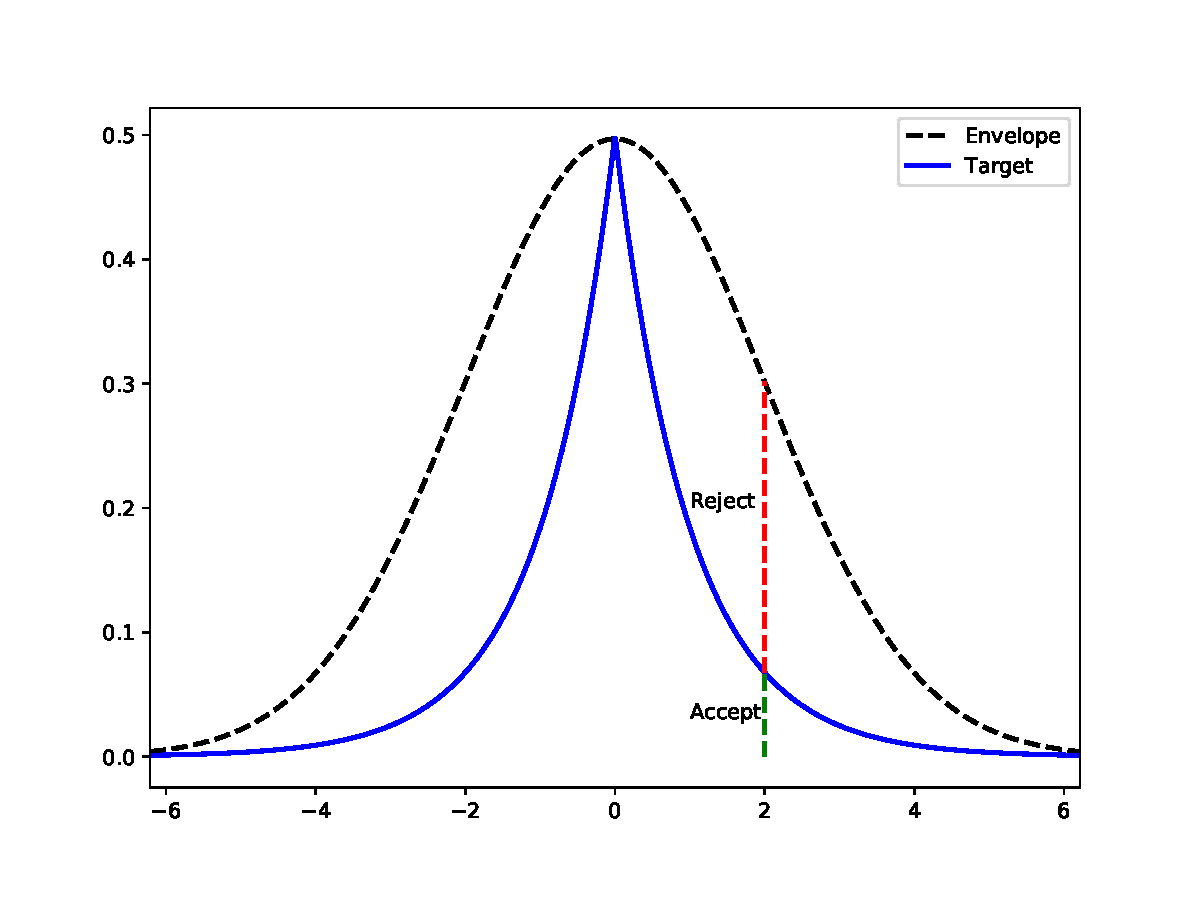
\includegraphics[scale=0.5]{fig1.pdf}


\begin{lstlisting}
# lests estimate this posterior using rejection sampling
def rejection_sampling():
while True:
# Re-use global parameters from above
x = np.random.normal(0, 2)
envelope = M * norm.pdf(x)
p = np.random.uniform(0, envelope)
if p < dg.pdf(x):
return x

# Generation samples from rejection sampling algorithm
samples = [rejection_sampling() for x in range(10000)]

# Plot Histogram vs. Target PDF
df['Target'].plot(color='blue', style='--', figsize=(8,6), linewidth=2.0)
pd.Series(samples).hist(bins=300, normed=True, color='green', 
alpha=0.3, linewidth=0.0)
plt.legend(['Target PDF', 'Rejection Sampling'])
\end{lstlisting}
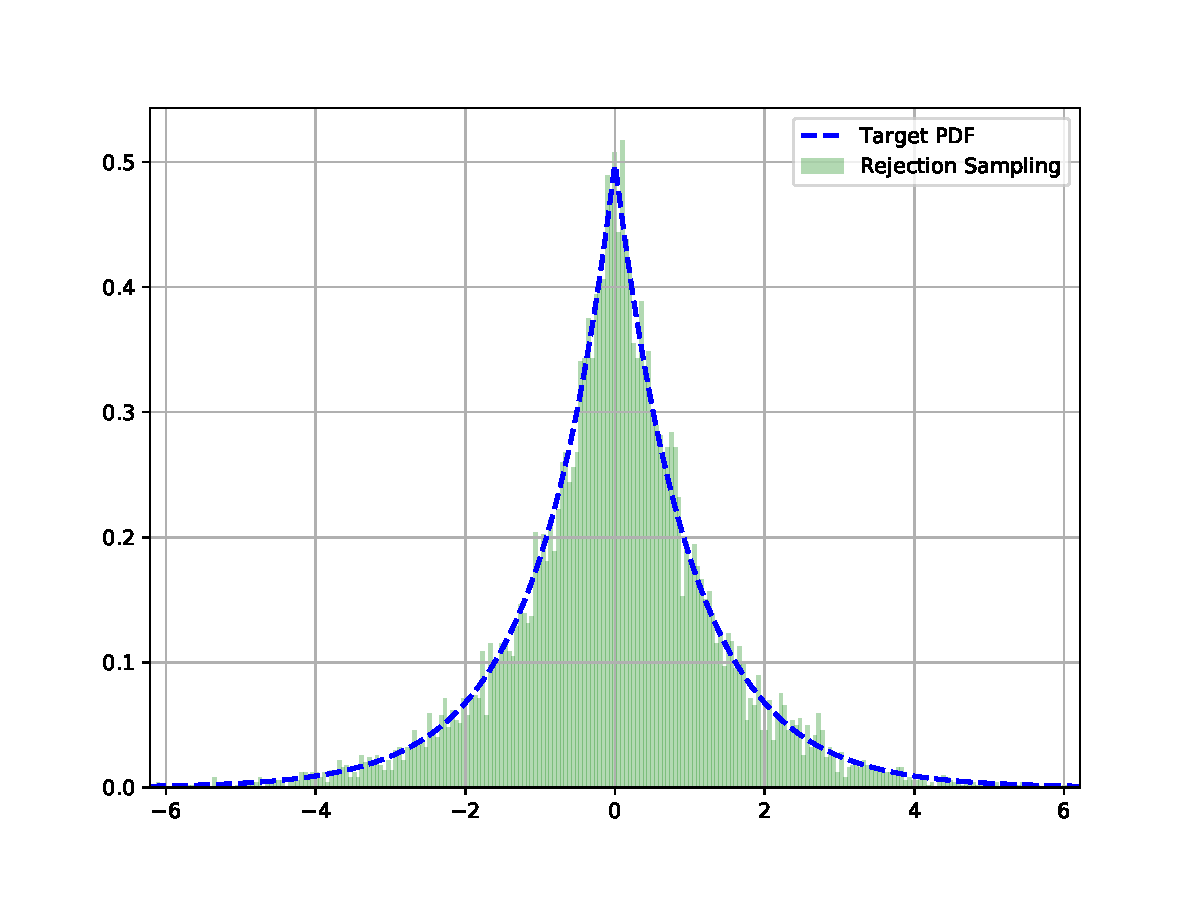
\includegraphics[scale=0.5]{fig2.pdf}
\end{document}
